\documentclass[8pt]{beamer}


\mode<presentation>
{

  \usetheme{Szeged} %use default if problems
  % or ... https://deic-web.uab.cat/~iblanes/beamer_gallery/index_by_theme.html
}

\usepackage{booktabs}
\usepackage{color}

\usepackage[english]{babel}
% or whatever

\usepackage[latin1]{inputenc}
% or whatever

\usepackage{times}
\usepackage[T1]{fontenc}
% Or whatever. Note that the encoding and the font should match. If T1
% does not look nice, try deleting the line with the fontenc.
\usepackage{nth}

\setbeamertemplate{caption}[numbered]


\title[S.I.s.a.R. Epidemic Model] % (optional, use only with long paper titles)
{The Contagion Sequences of the Epidemic S.I.s.a.R. Model: a Source of Suggestions for Intervention Policies}

\author[] % (optional, use only with lots of authors)
{G.~Pescarmona\inst{1} \and P.~Terna\inst{2} \and A.~Acquadro\inst{1} \and P.~Pescarmona\inst{3} \and G.~Russo\inst{4}  
\and S.~Terna\inst{5}  }
% - Give the names in the same order as the appear in the paper.
% - Use the \inst{?} command only if the authors have different
%   affiliation.


\institute[] % (optional, but mostly needed)
{
  \inst{1}%
 University of Torino, Italy
  \and
  \inst{2}%
  University of Torino, Italy, retired \& Collegio Carlo Alberto, Italy
 \and
  \inst{3}%
  University of Groningen, The Netherlands  
  \and
  \inst{4}%
  Centro Einaudi, Torino, Italy
  \and
  \inst{5}%
 tomorrowdata.io
  }
% - Use the \inst command only if there are several affiliations.
% - Keep it simple, no one is interested in your street address.


\date[] % (optional, should be abbreviation of conference name)
{Sep \nth{16}---Social Simulation Week 2020}

\begin{document}

%%%%%%%%%%%%%%%%%%%%%%%%%%%%%%%%%%%%%%%%%%%%%%%%%%%%%%%%%
\begin{frame}
  \titlepage
\end{frame}

%%%%%%%%%%%%%%%%%%%%%%%%%%%%%%%%%%%%%%%%%%%%%%%%%%%%%%%%%
%\begin{frame}{Outline}
%  \tableofcontents
  % You might wish to add the option [pausesections]
%\end{frame}

%%%%%%%%%%%%%%%%%%%%%%%%%%%%%%%%%%%%%%%%%%%%%%%%%%%%%%%%%
\section{Introduction}

%%%%%%%%%%%%%%%%%%%%%%%%%%%%%%%%%%%%%%%%%%%%%%%%%%%%%%%%%
\begin{frame}{Objectives of the Model}

  \begin{itemize}
  \item
We propose an agent-based model to simulate the Covid-19 epidemic diffusion, with Susceptible, Infected, symptomatic, asymptomatic, and Recovered people: hence the name S.I.s.a.R. The scheme comes from S.I.R. models, with (i) infected agents categorized as symptomatic and asymptomatic and (ii) the places of contagion specified in a detailed way, thanks to agent-based modeling capabilities. 

 \item
The infection transmission is related to three factors: the infected person's characteristics and the susceptible one, plus those of the space in which contact occurs.

  \item
The model includes the structural data of Piedmont, an Italian region, but it can be readily calibrated it for other areas. The model reproduces a realistic calendar (e.g., national or local government decisions), via its script interpreter.  

\bigskip

 \item
 
S.I.s.a.R. is at \url{https://terna.to.it/simul/SIsaR.html} with information on model costruction, the draft of a paper also reporting results, and an online executable version of the simulation program, built using NetLogo.

 \end{itemize}
\end{frame}

%%%%%%%%%%%%%%%%%%%%%%%%%%%%%%%%%%%%%%%%%%%%%%%%%%%%%%%%%
\section{Contagion Representation}

%%%%%%%%%%%%%%%%%%%%%%%%%%%%%%%%%%%%%%%%%%%%%%%%%%%%%%%%%
\subsection{The Proposed Technique}

%%%%%%%%%%%%%%%%%%%%%%%%%%%%%%%%%%%%%%%%%%%%%%%%%%%%%%%%%
\begin{frame}{Contagion Representation}

  \begin{itemize}
  \item
The model allows analyzing the sequences of contagions in simulated epidemics, while taking in account the places where they occur. 
  \item
We represent each infecting agent as a horizontal segment with a vertical connection to another agent receiving the infection. 
We represent the second agent via a further segment at an upper layer. 

  \item
With colors, line thickness, and styles, we display multiple data. 

  \item
This enables understanding at a glance how an epidemic episode is developing. In this way, it is easier to reason about countermeasures and, thus, to develop intervention policies.

  \end{itemize}
\end{frame}


%%%%%%%%%%%%%%%%%%%%%%%%%%%%%%%%%%%%%%%%%%%%%%%%%%%%%%%%%
\subsection{Significant Sequence Examples}

%%%%%%%%%%%%%%%%%%%%%%%%%%%%%%%%%%%%%%%%%%%%%%%%%%%%%%%%%
\begin{frame}{Contagion Sequences}

In Fig. \ref{fourSequences} we can look both at the places where contagions occur and at the dynamics emerging with different levels of intervention. 

\begin{figure}[H]
\center
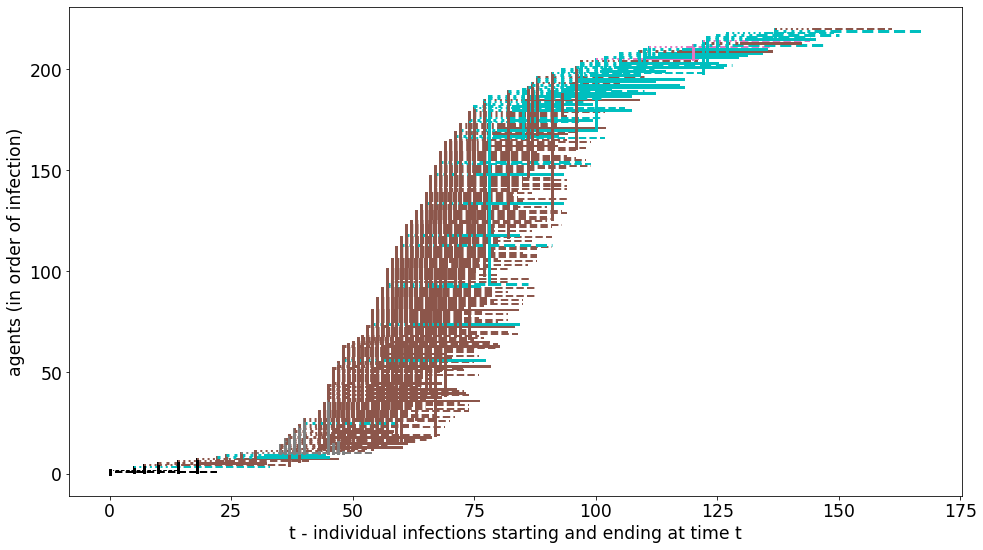
\includegraphics[scale=0.105]{withShort1.png}~~~~~~~~~~~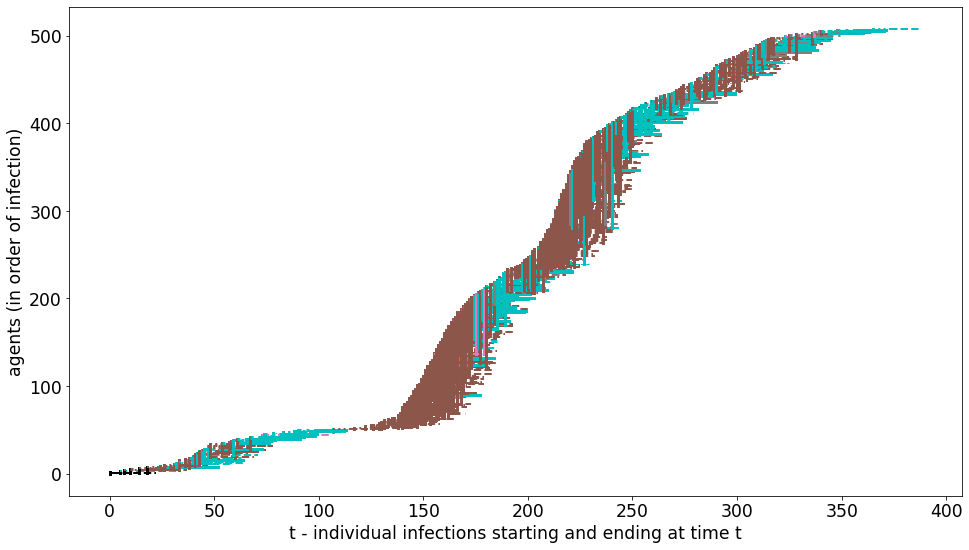
\includegraphics[scale=0.105]{withShort1A.png} 

\center
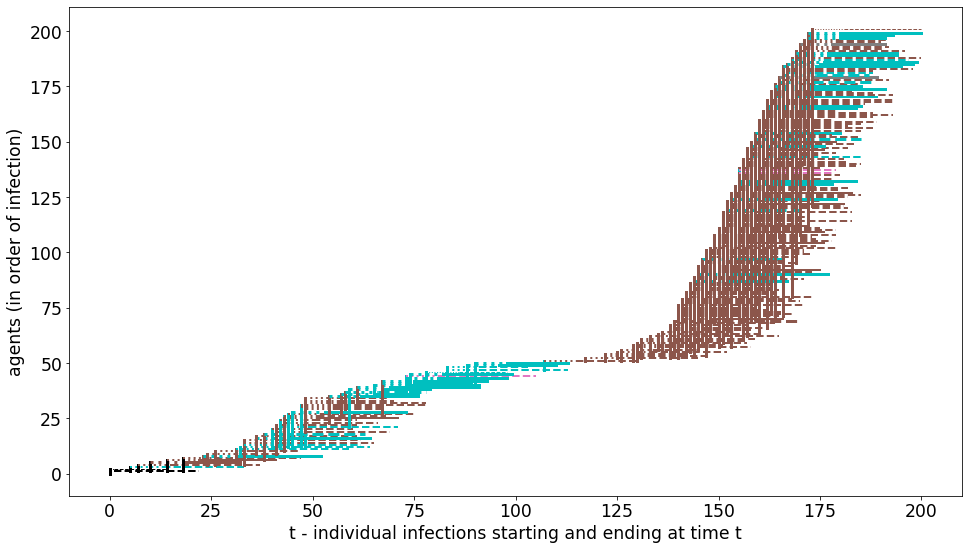
\includegraphics[scale=0.105]{withShort1A200.png}~~~~~~~~~~~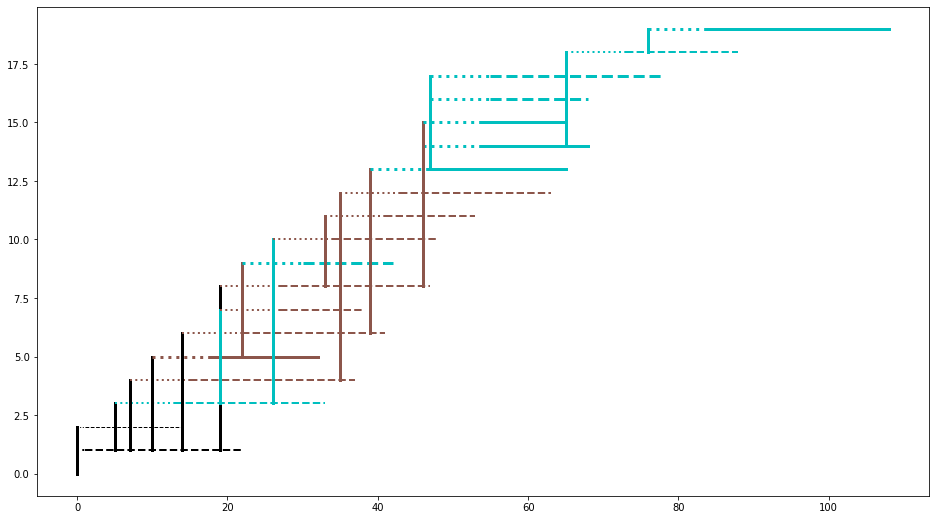
\includegraphics[scale=0.105]{withShort1B.png} \\
\caption{(\emph{top left}) an epidemic with containment measures, showing a highly significant effect of workplaces (brown);
 (\emph{top right}) the effects of stopping fragile workers at day 20, with a positive result, but home contagions (cyan) keep alive the pandemic, exploding again in workplaces (brown); (\emph{bottom left}) the same analyzing the first 200 infections with evidence of the event around day 110 with the new phase due to a unique asymptomatic worker, and (\emph{bottom right}) stopping fragile workers and any case of fragility at day 15, also isolating nursing homes} 
\label{fourSequences}
\end{figure}

\end{frame}

%%%%%%%%%%%%%%%%%%%%%%%%%%%%%%%%%%%%%%%%%%%%%%%%%%%%%%%%%
\section{Simulation Batches and Heat-Maps}

%%%%%%%%%%%%%%%%%%%%%%%%%%%%%%%%%%%%%%%%%%%%%%%%%%%%%%%%%
\subsection{Batches}

%%%%%%%%%%%%%%%%%%%%%%%%%%%%%%%%%%%%%%%%%%%%%%%%%%%%%%%%%
\begin{frame}{Batches}

  \begin{itemize}
  \item

We explore systematically the introduction of factual, counterfactual, and prospective interventions to control the spread of the contagions. 

  \item
Each simulation run---whose length coincides with the disappearance of symptomatic or asymptomatic contagion cases---is a datum in a wide scenario of variability in time and effects.   
  
  \item
  
Consequently, we need to represent compactly the results  emerging from batches of repetitions, to compare each batch's basic assumption's consequences.

 \item
We used blocs of one thousand repetitions. Besides summarizing the results with the usual statistical indicators, we adopted the technique of the heat-maps.

\end{itemize}
\end{frame}

%%%%%%%%%%%%%%%%%%%%%%%%%%%%%%%%%%%%%%%%%%%%%%%%%%%%%%%%%
\subsection{Two Heat-Maps}

%%%%%%%%%%%%%%%%%%%%%%%%%%%%%%%%%%%%%%%%%%%%%%%%%%%%%%%%%
\begin{frame}{Two Quite Different Heat-Maps for the Piedmont Region}

In Fig. \ref{2HM} we have two heat-maps reporting the duration of each simulated epidemic in the $x$ axis and the number of the symptomatic, asymptomatic, and deceased agents in the $y$ axis. 1,000 runs in both cases.

\begin{figure}[H]
\center
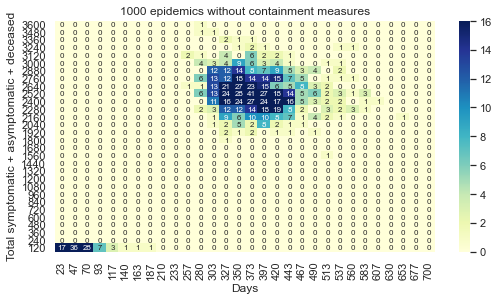
\includegraphics[scale=0.3]{HM30_readRunResults1k_noControl_plusHM.png}~~~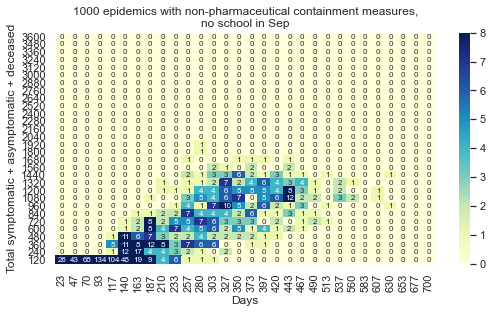
\includegraphics[scale=0.3]{HM30_readRunResults1k_withControl_plusHM.png} 

\caption{(\emph{on the left}) Epidemics without containment measures;
 (\emph{on the right}) Epidemics with basic non-pharmaceutical containment measures, no school in September 2020} 
\label{2HM}
\end{figure}

The actual Piedmont, where the curve of the contagions flattened with the end of May, with around 30 thousand subjects, is included in the cell in the first row, immediately to the right of the mode in Fig. \ref{2HM}, \emph{right side}.

\end{frame}


%%%%%%%%%%%%%%%%%%%%%%%%%%%%%%%%%%%%%%%%%%%%%%%%%%%%%%%%%
\section{Policies and Results}


%%%%%%%%%%%%%%%%%%%%%%%%%%%%%%%%%%%%%%%%%%%%%%%%%%%%%%%%%
\begin{frame}{Different Intervention Policies and Results}

\begin{table}[H]
\center
\footnotesize
%\small
\begin{tabular}{lrrrrr}
\toprule
Scenarios                              &  total sym.  & total sym.,       & days~~~~  \\
{}                                           &                    & asympt., deceased   \\                               
\midrule
1.~no control                       &  {\color{red}851.12}~     &  {\color{red}2253.48}         &  340.10~  \\
                                            &  (288.52)    &  (767.58)         &  (110.21) \\
\midrule
2.~basic controls, no           &   {\color{blue}158.55}~    &  {\color{blue}416.98}~         &  196.97~  \\
 school in Sep 2020            &   (174.10)     &  (462.94)        &  (131.18) \\
\midrule
3.~basic controls, \emph{schools}   &   {\color{blue}153.71}~    &       {\color{blue}409.73}~       &  199.35~  \\
 \emph{open} in Sep 2020                &  (168.55)   &     (454.12)        &  (129.00) \\
\midrule
4.~basic controls, \textbf{stop  fragile workers},   &   {\color{orange}120.17}~   &      {\color{orange}334.68}~         &  181.10~   \\
 no  schools in Sep 2020                          &   (149.10)  &     (413.90)         &   (125.46) \\
\midrule
%5.~basic controls, nursing homes isol.,    &  150.53~     &     408.08~         &  201.76~   \\
%no schools in Sep 2020                           &   (172.48)    &     (467.54)         &  (138.15) \\
%\midrule
%6.~basic controls, stop  fragile people,     &   154.15~    &     408.50~         &  195.81~  \\
%no   schools in Sep 2020                          &   (170.22)    &      (456.08)        &  (129.52) \\
%\midrule
5.~basic controls, \textbf{stop f. workers \&  f. people \&}    & \textbf{{\color{orange}105.63}}~    &  \textbf{{\color{orange}302.62}}~      &  174.39~   \\
\textbf{ n. h. isol}., no sch, Sep.                                              &   (134.80)   &     (382.14)          &  (121.82) \\
 \midrule
6.~b. controls, stop f. workers \&  f. people \& nur. h. isol.,  &  124.10~    &    397.05~           &  200.31~    \\
\& \textbf{factories op.}, no sch. Sep.                                               &  (132.42)   &    (399.64)           &  (121.46) \\
\midrule
7.~b. controls, stop f. workers  \&  f. people \& nur. h. isol.,   &  116.55~   &    374.68~           &  195.28~    \\
 \& \textbf{factories op., sch. open} Sep.                                            &  (130.91) &     (394.66)           &  (119.33) \\
\bottomrule
\end{tabular}
\caption{Report of the key results, with mean and (std)}
\label{keyResultsT}
\end{table}



\end{frame}

%%%%%%%%%%%%%%%%%%%%%%%%%%%%%%%%%%%%%%%%%%%%%%%%%%%%%%%%%
\section{Q\&As}

%%%%%%%%%%%%%%%%%%%%%%%%%%%%%%%%%%%%%%%%%%%%%%%%%%%%%%%%%
\begin{frame}{Replies to Organizers' Questions}

\begin{itemize}

\item \textit{What can your work speak of and what is it or will it be silent about?}

\bigskip
It is a tool for comparative analyses, not forecasting (the enormous standard deviation values are intrinsic to the problem).
\bigskip
        
               %Can you describe how and why you think the border between the two can be moved or not?
        
\item \textit{How can your work be adapted to (or is relevant/useful for) another disease, crisis, context, \ldots}

\bigskip
If we speak of contagions, the model is highly parametric and more it will be: we plan to build a second version in Python, using 
\url{https://terna.github.io/SLAPP/}.

\bigskip
    
\item  \textit{How can a crisis calling for immediate simulation help be supported by your work?}

\bigskip
We could take a substantial advantage from the parametric structure of the model.
\bigskip

\end{itemize}
 

\end{frame}







\end{document}